\section{均匀介质的热力学性质}
\subsection{内能、焓、自由能和吉布斯函数的全微分}
热力学函数的全微分助记符如下:
\begin{center}
    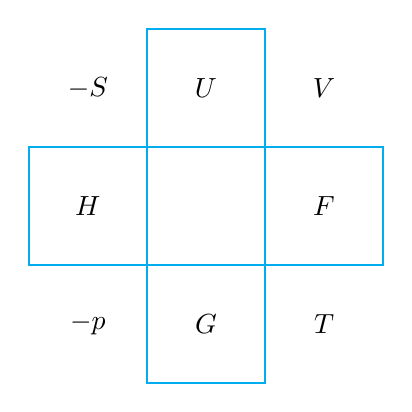
\begin{tikzpicture}[scale=1.5]
        \node at (0, -1) {$G$};
        \node at (-1, 0) {$H$};
        \node at (0, +1) {$U$};
        \node at (+1, 0) {$F$};
        \draw[cyan, thick] (-0.5, 1.5) rectangle (0.5, -1.5);
        \draw[cyan, thick] (-1.5, -0.5) rectangle (1.5, 0.5);
        \node at (-1, -1) {$-p$};
        \node at (-1, +1) {$-S$};
        \node at (+1, +1) {$V$};
        \node at (+1, -1) {$T$};
    \end{tikzpicture}
\end{center}
每个热力学函数的两边是其微分项(无需考虑正负号),而微分项对角线位置正好是各微分项对应的线性主部(需要考虑正负号). 以吉布斯函数$G$为例,其两边是微分项$\mathrm{d}p$和$\mathrm{d}T$,微分项的对角线位置是各自的线性主部$V$和$-S$,于是
$$
    \mathrm{d}G = V\mathrm{d}p - S\mathrm{d}T
$$
然后依次导出各热力学函数的全微分
\begin{equation}\label{吉布斯函数的全微分}
    \mathrm{d}G = V\mathrm{d}p - S\mathrm{d}T
\end{equation}
\begin{equation}\label{焓的全微分}
    \mathrm{d}H = T\mathrm{d}S - V\mathrm{d}p
\end{equation}
\begin{equation}\label{内能的全微分}
    \mathrm{d}U = T\mathrm{d}S - p\mathrm{d}V
\end{equation}
\begin{equation}\label{自由能的全微分}
    \mathrm{d}F = -p\mathrm{d}V - S\mathrm{d}T
\end{equation}



\subsection{麦克斯韦关系}
下面以吉布斯函数$G$为例,介绍各个热力学函数的麦克斯韦关系:首先根据吉布斯函数的全微分,写出其偏导数
$$
    \left(\frac{\partial G}{\partial p}\right)_T=V, \quad
    \left(\frac{\partial G}{\partial T}\right)_p=-S,
$$
由于$G$是连续函数,所以它的二阶混合偏导数必然相等
$$
    \left[\frac{\partial}{\partial T}\left(\frac{\partial G}{\partial p}\right)_T\right]_p = -\left[\frac{\partial}{\partial p}\left(\frac{\partial G}{\partial T}\right)_p\right]_T
$$
也即
$$
    -\left(\frac{\partial S}{\partial p}\right)_T=\left(\frac{\partial V}{\partial T}\right)_p
$$
类似地,我们能依次导出所有热力学函数的麦克斯韦关系
\begin{align}\label{麦克斯韦关系}
    -\left(\frac{\partial S}{\partial p}\right)_T & = \left(\frac{\partial V}{\partial T}\right)_p  \\
    \left(\frac{\partial T}{\partial p}\right)_S  & = \left(\frac{\partial V}{\partial S}\right)_p  \\
    \left(\frac{\partial T}{\partial V}\right)_S  & = -\left(\frac{\partial p}{\partial S}\right)_V \\
    \left(\frac{\partial p}{\partial T}\right)_V  & = \left(\frac{\partial S}{\partial V}\right)_T
\end{align}
这一切操作和变换,都是为了把无法通过实验直接测量的热力学函数$G, H, U, F$转化为可以通过实验直接测量的参量$p, S, V, T$.



\subsection{气体的节流过程和绝热膨胀过程}
\paragraph{节流过程}管子用不导热的材料制成,管子中间有一个多孔塞,多孔塞两边各维持着较高的压强$p_1$和较低的压强$p_2$,于是气体从高压的一边经过多孔塞不断地流向低压的一边,并达到定常状态.


\subsection{基本热力学函数的确定}